\noindent This research is inspired by the movement to strengthen urban neighborhoods that began in the previous century, but the context for this particular study stems from the recent global health crisis. Already, many scholars have addressed the urban challenges resulting from the COVID-19 pandemic. However, the specific goal of quantifying social gatherings in city parks has yet to be accomplished in existing studies. The literature review below provides initial insight into the concepts and methodologies used in the research that follows.\\

\begin{figure}[h]
  \centering
  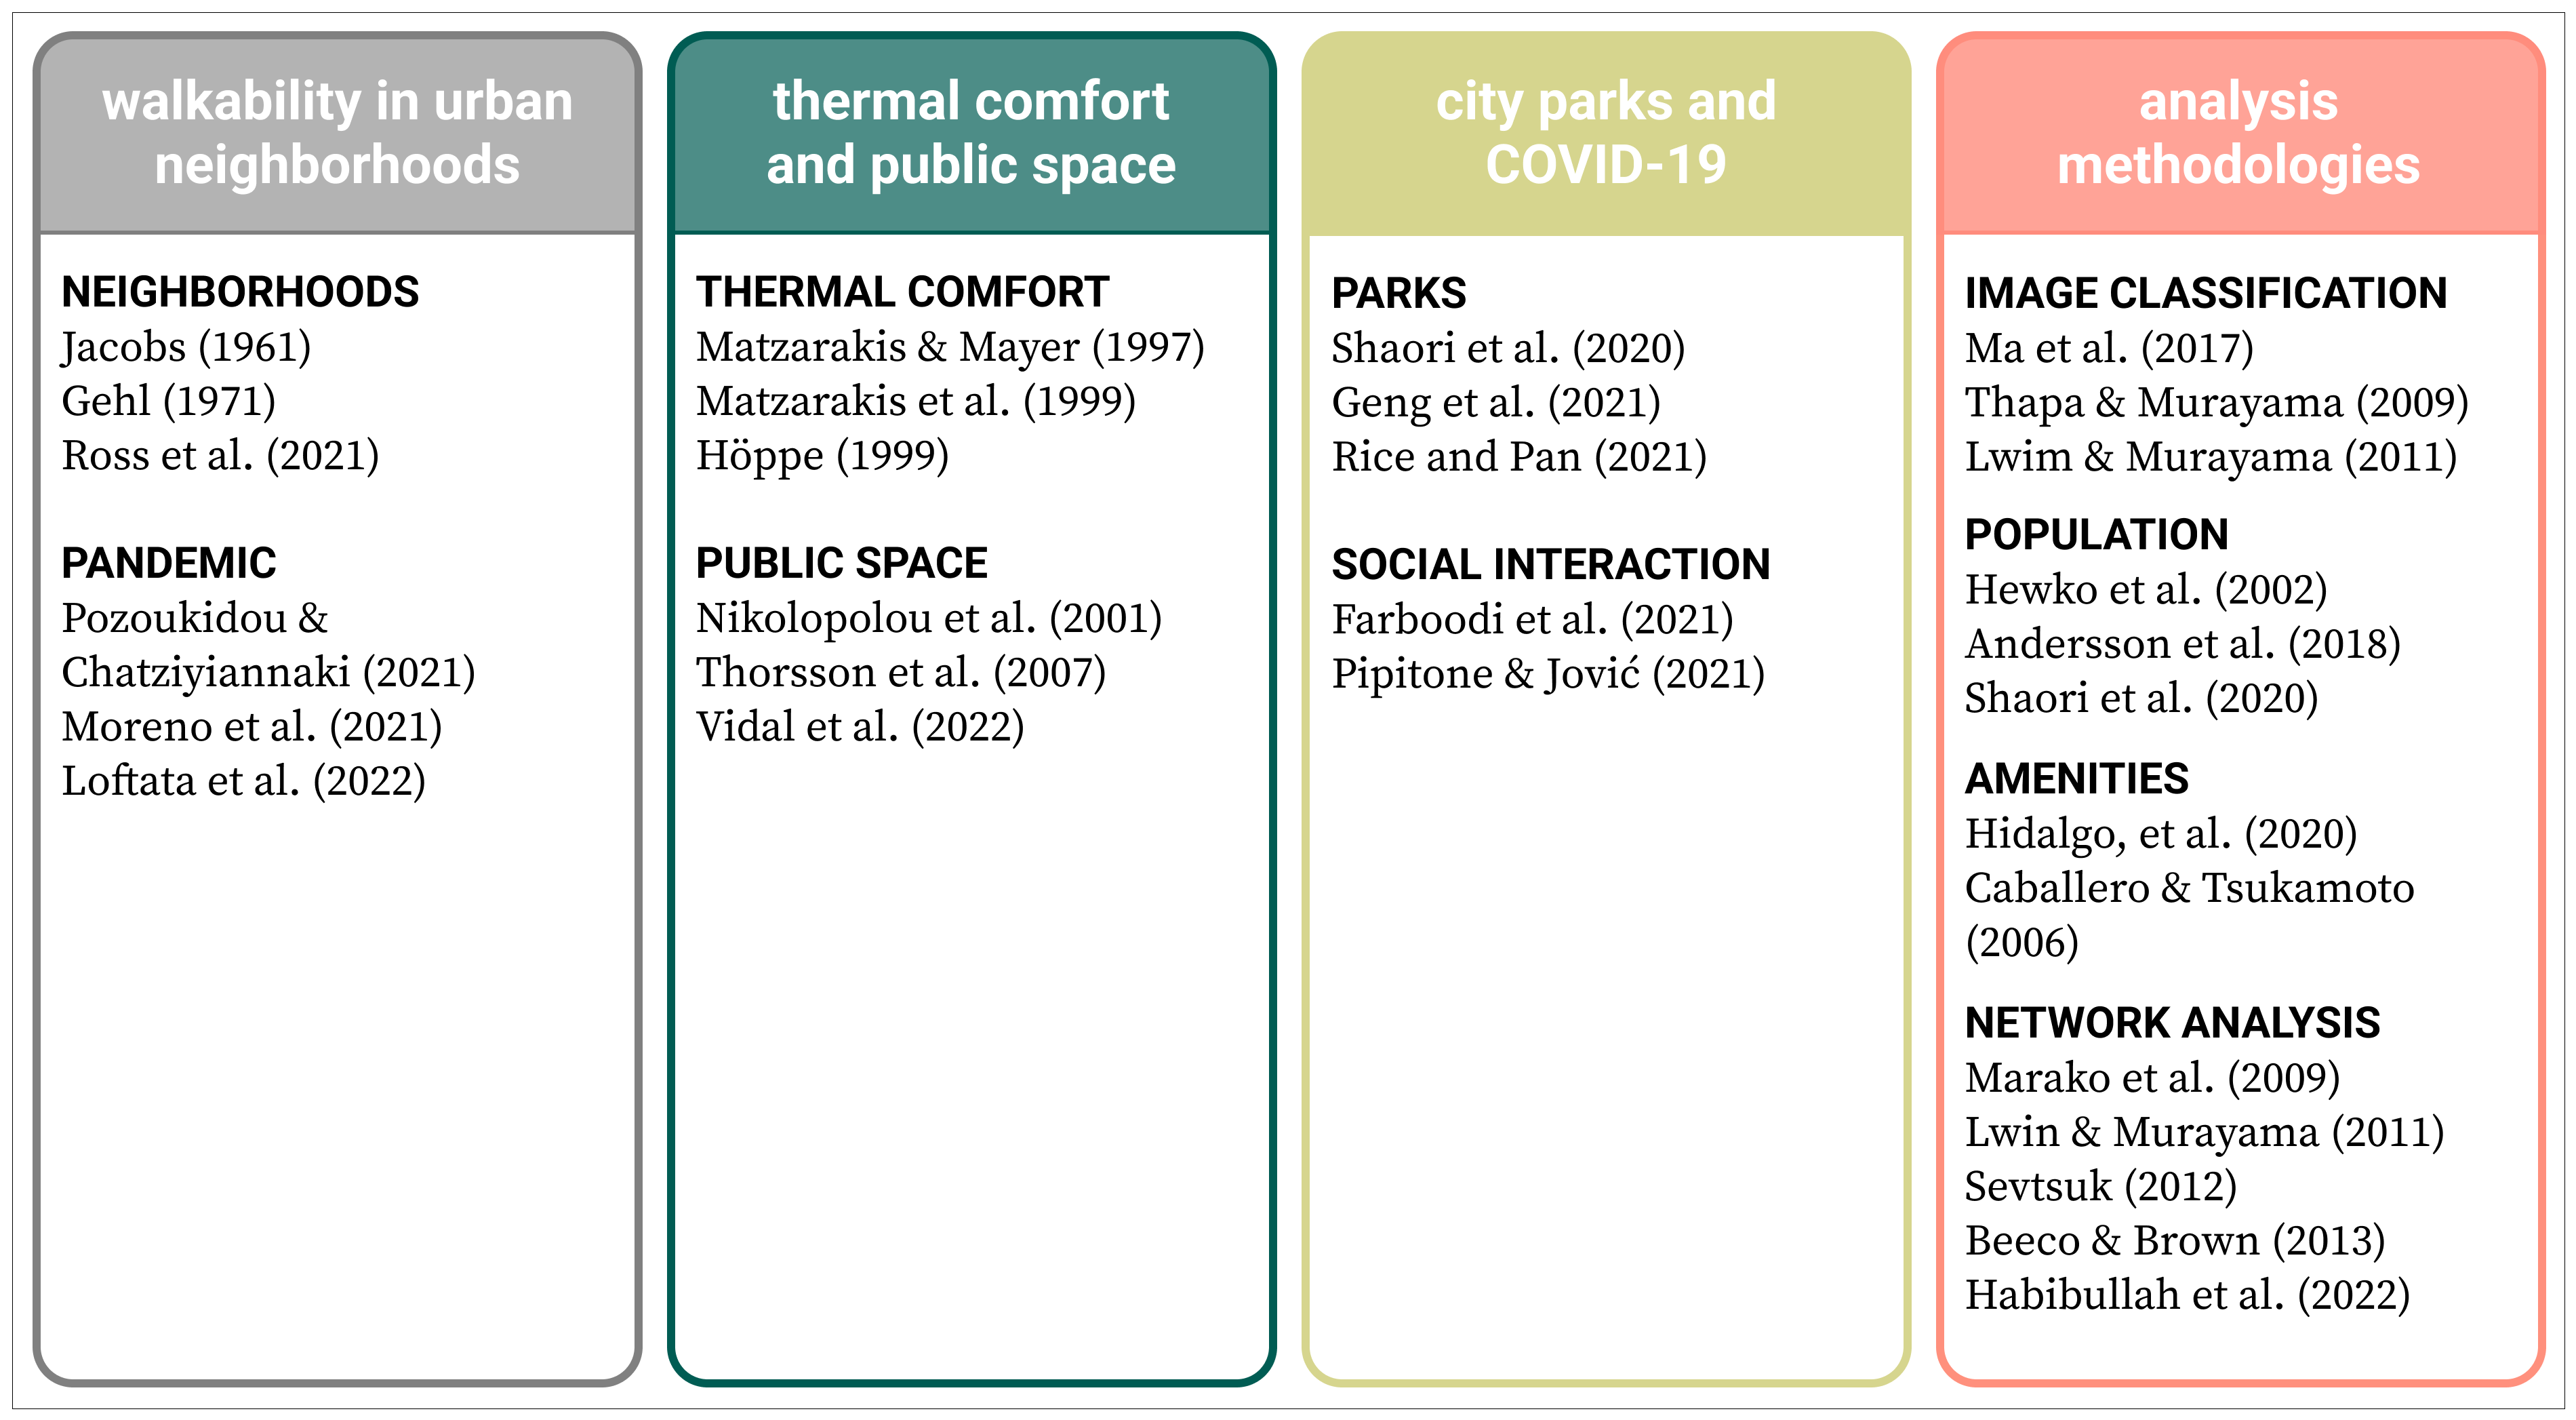
\includegraphics[width=1.0\textwidth]{images/literature/theory.png}
  \captionsetup{width=1.0\linewidth}
  \caption[Literature review]{Literature review themes and applicable references.}
  \label{fig:literature}
\end{figure}

\begin{multicols}{2}

\section{Walkability in urban neighborhoods}
From a perspective of safety and the context of urban exodus in the mid-twentieth century US, Jacobs (1961) writes that city neighborhoods should be planned to "foster lively and interesting streets," be a continuous network throughout a subsection of a city, and to function as districts in and of themselves. According to Jacobs, parks and public spaces should "knit together the [urban] fabric's complexity and multiple use" instead of isolating neighborhoods \cite{jacobs_death_2020}. Similarly, Gehl (2011) advocates for the \textit{lively} street, where people can see and be seen, a condition which increases the possibility for social interactions in the urban environment. Outdoor activities in the urban environment are divided into three categories by Gehl: necessary, optional, and social. Social activities "depend on the presence of others in public spaces" and the physical conditions of the environment directly influence pedestrian quantity, length of time spent outdoors, and the activities which occur \cite{gehl_life_2011}. 

More recently, but before the pandemic, a resurgence in the neighborhood movement was spearheaded by Carlos Moreno in 2016 with the "15-minute City" concept. The idea being that high-quality urban life is inversely proportional to time spent using transportation. Through density, diversity, digitalization and proximity of urban services, Moreno et al. (2021) propose interconnected neighborhoods where residents can meet their needs within a fifteen-minute pedestrian or cycling trip from home \cite{moreno_introducing_2021}. Separately, Ross et. al (2021) finds recreational walking to be one factor that contributes to individual "flourishing" in a neighborhood \cite{ross_walking_2021}. 

Pozoukidou and Chatziyiannaki (2021) write about the renewed importance of walkable cities in the face of the COVID-19 pandemic, and how cites around the world were actively making policy changes in the face of the public health crisis. The authors divide city policies into three pillars: inclusion, health and safety, and evaluate the overall proximity of amenities on a neighborhood scale \cite{pozoukidou_15-minute_2021}. Loftata et al. (2022) also cover the topic of neighborhood walkability and the social implications of COVID-19 pandemic restrictions. Their research employed surveys to understand the changing patterns of residents in cities around the world, finding that access to basic amenities by 15-20 minute walking distance and social cohesion became critical during the pandemic \cite{lotfata_changing_2022}. 

\section{Thermal comfort and public space}
The work of Matzarakis and Mayer (1997) and Matzarakis et al. (1999) relating physiological equivalent temperature (PET), thermal perception, and grade of physiological stress is significant when considering comfort in outdoor public spaces \cite{matzarakis_urban_1997}\cite{matzarakis_applications_1999}. Further, Höppe (1999) relates PET to air temperatures in the winter sun and shade and summer sun and shade, providing a point of reference for understanding the relationship between the two conditions. Using these concepts, many researchers have since conducted behavioral studies to understand how thermal comfort is experienced in public spaces. Nikolopolou et al. (2001) determined thermal neutrality of urban spaces in Cambridge, England to range from 7.5 degrees Celsius in the winter to 27 degrees Celsius in the summer, and further found that users eating and socializing preferred sunlight and warm conditions to shade \cite{nikolopoulou_thermal_2001}. 

Thorsson et al. (2007) studied temperature in relation to urban space in Japan using structured interviews, observations of behavior, and micrometeorological measurements to compare a public square and public park in the same town. The park was found to be cooler than the square, both in actual temperature measurement and in terms of calculated physiological equivalent temperature (PET) value. In addition, a relationship was found between the perceived thermal conditions and the amount of time the respondents spent in the public space \cite{thorsson_thermal_2007}.

Vidal et al. (2022) used the environmental psychology data collection technique called Behavioral Mapping (BM) to identify patterns of behavior in Public Urban Green Spaces (PUGS). Among other findings, the study shows that natural areas are less likely to be used than areas that are manicured or contain urban furniture like benches, and that sunny but not excessively hot days are the most desirable for using the public spaces. Their conclusion was therefore that future green space designs should use vegetation to shape the space, including clearings for picnics, and to integrate both sunny and shaded areas so that users can make a choice depending on the weather and their needs \cite{vidal_patterns_2022}. 

\section{City parks and COVID-19}
Geng et al. (2021) conducted a global study of pandemic impacts on park visitation, finding that in most countries park visitation increased after February 2020. Using stepwise regression analysis to compare daily confirmed cases of COVID-19, Google Mobility data on park visitation before and after the pandemic, and government policies relating to the public health crisis, it was found that stay-at-home orders and restrictions on public transportation were the most significant factors negatively correlated with changes to park visitation. Interestingly, the least significant factor was the daily increase in the number of known cases of COVID-19, showing that an increase in cases did not increase or decrease park visitation \cite{geng_impacts_2021}. 

Furthermore, the Geng et al. study includes the three the countries featured in this research: United States, England (UK), and Japan. For Japan---alongside Italy, Spain, South Korea, and Sweden---it was found that there was not a significant change to park visitation when COVID-19 began \cite{geng_impacts_2021}. The authors suggest that this was a result of the government response and restrictions, but the paper does not compare access to parks in any of the studied countries. It is possible that park visitation could not change during the pandemic in cities that do not have an abundance of accessible parks. 

Park visitation during the pandemic was also studied by Rice and Pan (2021) through Google's open-source mobility trend data, finding that season and age of population had an affect on park usage during the pandemic that mobility data did not account for. The authors call for park design that creates ample social distancing opportunities in order to improve the physical and social well-being of a population during a pandemic \cite{rice_understanding_2021}.

Shaori et al. (2020) study park space allocation per person for England and Wales when considering COVID-19 pandemic-related social distancing recommendations. The authors use 500 and 1000 meter buffers around postal codes to quantify per capita park space \cite{shoari_accessibility_2020}. The results found postal codes with four square meters of green space per person to be inadequate for meeting social distancing needs, likely leading to overcrowded parks. The study is important for analyzing park access on a national level, but using postal codes for population data can lead to aggregation error in the results. The research that follows uses smaller administrative boundaries and focuses on three specific parks to understand accessibility at a finer level of detail. 

Pipitone and Jović (2021) study equitable access to green space during pandemic conditions. Through online surveys they found that the COVID-19 pandemic expanded the socio-spatial inequities already present in New York City \cite{pipitone_urban_2021}. Also in the US, Farboodi et al. (2021), calculated the cost of social risk during the COVID-19 pandemic through cell phone tracking data and mobility reports. The study found that recreation activity in the US had recovered from the initial pandemic lockdown effects by July 1, 2020 \cite{farboodi_internal_2021}. Farboodi et al. conclude that individuals lowered their social activity in the first months of the pandemic to reduce the risk of infection, but since herd immunity is one solution to overcoming an infectious disease, people must weigh the risk of socializing on an individual level. 

\section{Analysis methodologies}
The research that follows will make use of several different spatial analysis methodologies. The first applied technique is object-based image classification, which uses aerial imagery for land-cover mapping. Ma et al. (2017) perform a meta-analysis on the research methodologies used in 173 scientific papers. According to their findings, the methodology of supervised object-based image classification is quickly advancing in the field, and an area-based method is found to be more accurate than the point-based method \cite{ma_review_2017}. 

Thapa and Murayama (2009) analyze image classification approaches for urban land use in the city of Tsukuba, Japan. The land use classes used by Thapa and Maruyama include urban forest, lawn/grass, paddy field, dry farmland/exposed field, facility/industry, residence/parking/road, and water. The four classification approaches used were unsupervised, supervised, fuzzy supervised, and GIS post-processing, which extracted the matching features from the first three approaches and was found to be the most accurate method \cite{thapa_urban_2009}. In the same city, Lwin and Murayama (2011) model urban green space through the combined methodology of remote sensing, GIS and spatial web technology. The resulting "eco-friendly walk score calculator" allows residents to determine either the shortest route (for shopping activities) or the greenest walking route (for recreational activities) \cite{lwin_modelling_2011}. 

Population studies are used to analyze the spatial distribution, amenity distribution, and population characteristics within a research area. The spatial distribution of age is analyzed by Andersson et al. (2018), finding the relationship between localized access to amenities and how the age of neighborhood reflects the priorities of people in that age group \cite{andersson_urban_2018}. As mentioned above, Shaori et al. (2020) used population data and park allocation to determine access to parks during the pandemic. In this study, population catchment will be analyzed to estimate the population of residents within walking distance to a park compared to the social gathering capacity within the park. 

The distribution of urban amenities is a widely-studied topic using a variety of methodologies. Hidalgo et al. (2020) use spatial analysis techniques to find amenities that are over and under supplied in neighborhoods throughout the US. Clustering algorithms identify neighborhoods by amenity density, and then the model compares predicted versus actual number of amenities. The authors find in cities like Tokyo and London, amenities cluster around transit stations due to the number of daily riders, but "exogenous destinations" that also attract amenities include dense residential or employment areas, busy intersections, and public facilities and open spaces \cite{hidalgo_amenity_2020}.

Caballero and Tsukamoto (2006) discuss the concept of "dividual space," which is the idea of private physical spaces within commercial facilities in Tokyo. The authors propose that public space is not equivalent to "collective" space, which is why amenities like karaoke and internet cafes that provide space to rent by the hour for individuals or small groups are popular across Japan \cite{caballero_tokyo_2006}. This supports the pandemic-driven concept of social gathering spaces that are available for use by individuals and small groups in the research that follows. 

Beeco and Brown (2013) review methodologies for finding the capacity of parks and protected areas (PPA) to allow for use without a resource deteriorating due to the quantity of visitors. The authors describe the different needs of trail users who seek out established trail routes compared to "urban socials" who need urban parks for large social gatherings \cite{beeco_integrating_2013}. In other words, from the perspective of resource conservation, the capacity of natural spaces should be determined to prevent overuse and deterioration of the environment. 

Spatial access to public open space (POS) during the recent pandemic is analyzed by Habibullah et al. (2022), by quantifying park access within a one-kilometer walking distance in the city of Jeddah, Saudi Arabia. The public open spaces are categorized by average area including local/pocket, neighborhood, district/city, regional, and national/metropolitan parks. Analyzed by district, the results show the percentage of the population that had access to public open space within one kilometer \cite{habibullah_one-kilometer_2022}.  

Marako et al. (2009) write about the complications of determining access to parks in New York City. Their findings reveal parks to not be equitably distributed geographically, meaning the ability for residents to be physically active is not geographically equal across the city. Further, they emphasize the importance of using entry points to measure access because a neighborhood can border a park without there being a way to physically enter the space \cite{maroko_complexities_2009}. In other words, the entry points of parks might reveal a lack of access despite proximity to certain neighborhoods.

\section{Originality}
A substantial amount of research has been conducted on parks, neighborhood amenities, COVID-19, and some combination of those three topics. However, there does not seem to be existing research quantifying outdoor social gatherings in city parks. Moreover, there does not appear to be research assessing the accessibility of social gatherings in parks while considering food amenities and the surrounding population. This research will make use of methodologies similar to those used in the above existing research, especially the combined use of image classification and network analysis methodology implemented by Lwin and Murayama (2011). This study aims to contribute to the growing literature on access to city parks, with access being important both in times of “normalcy” and during a public health crisis. 

\end{multicols}

